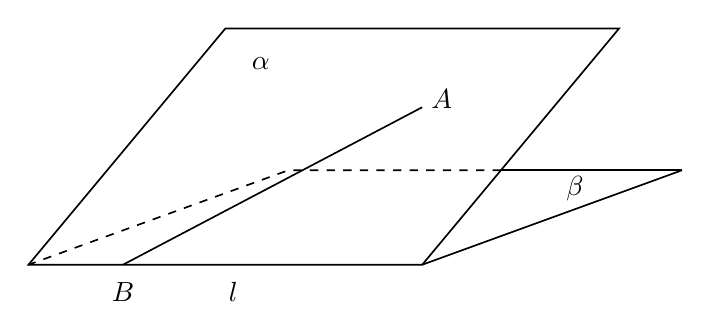
\begin{tikzpicture}[x=1cm,y=1cm,font=\normalsize,line width=.6pt]
\coordinate (L) at (-4.50,0.00);
\coordinate (Rb) at (0.50,0.00);
\coordinate (Rt) at (3.00,3.00);
\coordinate (Lt) at (-2.00,3.00);
\coordinate (Bpt) at (-3.3,0);
\coordinate (Apt) at (0.50,2.00);
\coordinate (K) at (-1.20,1.20);
\coordinate (Mr) at (-1.2,1.2);
\coordinate (Fr) at (3.8,1.2);
% plane alpha outline
\draw[solid] (L) -- (Rb) -- (Rt) -- (Lt) -- cycle;
% plane beta: front edges solid
\draw[solid] (Rb) -- (Fr);
% hidden intersection segments dashed
\coordinate (V) at (1.5,1.2);
\draw (Fr)--(V);
\draw[dashed] (V)--(K)--(L);
% skew line AB in alpha
\draw[solid] (Bpt) -- (Apt);
\node[inner sep=2pt] at (-1.55,2.55) {$\alpha$};
\node[inner sep=2pt,xshift=-6.00bp,yshift=2.00bp] at (2.65,0.9) {$\beta$};
\node[inner sep=2pt,above=3pt,right=1pt] at (Apt) {$A$};
\node[inner sep=2pt,below=4pt] at (Bpt) {$B$};
\node[inner sep=2pt,below=4pt] at (-1.90,0.00) {$l$};
\end{tikzpicture}
